\documentclass[tikz]{standalone}
\newcommand{\vect}{\mathbf}
\newcommand{\uf}{\vect{u}_f}
\newcommand{\Opp}{\mathrm{Opp}}
\newcommand{\Sf}{\vect{S}_f}
\newcommand{\Mag}[1]{\lvert #1 \rvert}
\newcommand{\magSf}{\Mag{\Sf}}
\newcommand{\vol}{\mathcal{V}}

\usetikzlibrary{plotmarks}
\usetikzlibrary{patterns}
\begin{document}
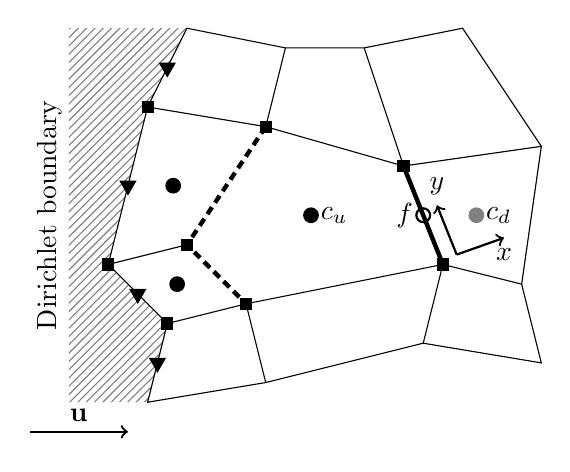
\begin{tikzpicture}[
  scale=0.25,
  cpnt/.style={fill=black},
]
\fill [pattern=north east lines,pattern color=gray] (5,0) -- (6,4) -- (3,7) -- (5, 15) -- (7,19) -- (1,19) -- (1,0);
\node at (0,9.5) {\rotatebox{90}{Dirichlet boundary}};

\draw [white] (-1,-2.1) rectangle (-1,-2);
\draw [thick, ->] (-1,-1.5) -- (4,-1.5) node [midway, anchor=south] {$\vect{u}$};

\draw [thick, ->] (20.7,7.5) -- (19.7,10) node [at end, anchor=south] {$y$};
\draw [thick, ->] (20.7,7.5) -- (23.1,8.35) node [at end, anchor=north] {$x$};

\draw (10,5) -- (20,7) -- (18,12) -- (11,14);
\draw [densely dashed, ultra thick] (11,14) -- (7,8) -- (10,5);
\draw [ultra thick] (20,7) -- (18,12);
\draw [thick] (19,9.5) circle [radius=0.35] node [anchor=east] {$f$};
\path [cpnt] (13.3,9.5) circle [radius=0.4] node [anchor=west, black] {$c_u$};
\path [fill=gray] (21.7,9.5) circle [radius=0.4] node [anchor=west, black] {$c_d$};

% direct upwind cells
\draw (10,5) -- (6,4) -- (3,7) -- (7,8);
\path [cpnt] (6.5,6) circle [radius=0.4];

\draw (3,7) -- (5,15) -- (11,14);
\path [cpnt] (6.3,11) circle [radius=0.4];

\draw (20,7) -- (24,6) -- (25,13) -- (18,12);
\draw (20,7) -- (19,3) -- (25,2) -- (24,6);
\draw (19,3) -- (11,1) -- (10,5);
\draw (11,14) -- (12,18) -- (16,18) -- (18,12);
\draw (16,18) -- (21,19) -- (25,13);
\draw (5,15) -- (7,19) -- (12,18);
\draw (6,4) -- (5,0) -- (11,1);

% vertices
\node at (3,7) {\pgfuseplotmark{square*}};
\node at (5,15) {\pgfuseplotmark{square*}};
\node at (11,14) {\pgfuseplotmark{square*}};
\node at (18,12) {\pgfuseplotmark{square*}};
\node at (10,5) {\pgfuseplotmark{square*}};
\node at (20,7) {\pgfuseplotmark{square*}};
\node at (6,4) {\pgfuseplotmark{square*}};
\node at (7,8) {\pgfuseplotmark{square*}};
\node at (5.5,2) [scale=1.5,rotate=60] {\pgfuseplotmark{triangle*}};
\node at (6,17) [scale=1.5,rotate=60] {\pgfuseplotmark{triangle*}};
\node at (4,11) [scale=1.5,rotate=60] {\pgfuseplotmark{triangle*}};
\node at (4.5,5.5) [scale=1.5,rotate=60] {\pgfuseplotmark{triangle*}};
\end{tikzpicture}
\end{document}
